%MẪU LÀM CÂU HỎI TỰ LUẬN
%Dùng với gói lệnh lamdethi.sty
%Dùng Vietex 2.8. với phông mã Unicode
%Người soạn : Nguyễn Hữu Điển, ĐHKHTN, ĐHQG HN
%Mail: huudien@vnu.edu.vn, CQ: (84 - 4) 557 2869
%NR: (84 - 4) 641 8848, DĐ: 0989061951
%Ngày 26/12/2009
%%%%%%%%%%%%%%%%%%%%%%%%%

\baituluan{logic:1}{%Câu hỏi 1

Tìm giá trị của $a_2+a_4+a_6+...+a_{98}$ nếu $a_1, a_2, a_3, ...$ là một cấp số cộng với công sai $1$ và $a_1+a_2+a_3+...+a_{98}=137$.
}{%Trả lời

Tổng của một cấp số cộng là tích của số các số hạng với trung bình cộng của tổng của số hạng đầu và số hạng cuối . Vì vậy, $a_1+a_2+...+a_{98}=98\left(\dfrac{a_1+a_{98}}{2}\right)=49(a_1+a_{98})=137$. Tương tự, $a_2+a_4+...+a_{98}=49\left(\dfrac{a_2+a_{98}}{2}\right)=49\left(\dfrac{a_1+1+a_{98}}{2}\right)=\dfrac{49(a_1+a_{98})}{2}+\dfrac{49}{2}=93$ 

\textit{Cách làm khác}: Tách riêng các số hạng có chỉ số lẻ và chẵn, đặt $S_o=a_1+a_3+...+a_{97}$ và $S_e=a_2+a_4+...+a_{98}$. Khi đó, mỗi dãy có $49$ số hạng và từ $a_{n+1}=a_n+1$ với mọi $n\ge 1$, ta có $S_o=S_e-49$. Hơn nữa, $S_e+S_o=137$. Thay $S_o$ vào phương trình trên và giải $S_e$, ta tìm được $S_e=93$

\textbf{Đáp án: $93$}
}%Hết câu hỏi 1


\baituluan{logic:2}{%Câu hỏi 2

Số nguyên $n$ là một bội số nguyên dương nhỏ nhất của $15$ mà mỗi chữ số của nó là $0$ hoặc $8$. Tính $\dfrac{n}{15}$.
}{%Trả lời

Lưu ý rằng $n$ là bội chung của $5$ và $3$. Vì $n$ là bội c $5$ nên $n$ phải kết thúc bằng $0$, chữ số $5$ không thỏa mãn đề bài. Vì $n$ là bội của $3$ nên $n$ phải chứa chữ số $8$ sao cho tổng là bội của $3$. Vì vậy, theo yêu cầu của đề bài, $n=8880$ và $\dfrac{8880}{15}=592$ là đáp án của bài toán.

\textbf{Đáp án: $592$}
}%Hết câu hỏi 2

\baituluan{logic:3}{%Câu hỏi 3

$P$ là một điểm nằm trong $\triangle ABC$ sao cho các đường thẳng đi qua $P$ và song song với các cạnh của $\triangle ABC$ tạo thành các tam giác nhỏ $t_1, t_2$ và $t_3$ có diện tích tương ứng là $4, 9$ và $49$. Hãy tìm diện tích của $\triangle ABC$. 
\begin{center}
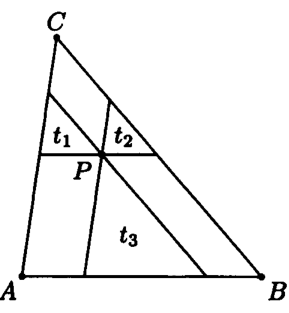
\includegraphics[scale=0.7]{hinhc3}  
\end{center}  
}{%Trả lời

Đặt $T$ là diện tích của $\triangle ABC$ và $T_1, T_2$ và $T_3$ lần lượt là diện tích của các tam giác $t_1, t_2$ và $t_3$. 

Đặt $c$ là độ dài cạnh $AB$ và $c_1, c_2$ và $c_3$ lần lượt là độ dài của các cạnh song song với $AB$ của $t_1, t_2$ và $t_3$. Khi đó, không mất tính tổng quát, trong mỗi tam giác có:
\begin{center}
$\dfrac{\sqrt{T_1}}{\sqrt{T}}=\dfrac{c_1}{c}, \dfrac{\sqrt{T_2}}{\sqrt{T}}=\dfrac{c_2}{c}$ và $\dfrac{\sqrt{T_3}}{\sqrt{T}}=\dfrac{c_3}{c}$.
\end{center}
Hơn nữa, từ $c_1+c_2+c_3=c$, ta có:
$\dfrac{\sqrt{T_1}}{\sqrt{T}}+\dfrac{\sqrt{T_2}}{\sqrt{T}}+\dfrac{\sqrt{T_3}}{\sqrt{T}}=\dfrac{c_1+c_2+c_3}{c}=1$.

Vì thế, $T=(\sqrt{T_1}+\sqrt{T_2}+\sqrt{T_3})^2=(\sqrt{4}+\sqrt{9}+\sqrt{49})^2=144$.

\textbf{Đáp án: $144$}
}%Hết câu hỏi 3
\baituluan{logic:4}{%Câu hỏi 4

Cho $S$ là một tập hợp các số nguyên dương - không nhất thiết phải phân biệt - có số $68$. Trung bình cộng các số trong $S$ là $56$. Tuy nhiên, nếu không có số $68$, trung bình cộng các số còn lại là $55$. Hỏi số nào là số lớn nhất trong $S$?
}{%Trả lời

 Đặt $n$ là các số nguyên dương trong $S$ và $m$ là tổng của chúng. Theo đề bài ta có: 
\begin{center}
$\dfrac{m}{n}=56$ và $\dfrac{m-68}{n-1}=55$.
\end{center}
Giải đồng thời các phương trình trên ta được $n=13$ và $m=728$.
Bây giờ, để tối đa hóa phần tử lớn nhất của $S$, ta phải giảm thiểu các phần tử khác. Như vậy, $S$ phải chứa $11$ số $1$, $1$ số $68$ và $1$ số $649$, bởi $728-11-68=649$.

\textbf{Đáp án: $649$}
}%Hết câu hỏi 4

\baituluan{logic:5}{%Câu hỏi 5

Xác định giá trị của $ab$ biết $\log_8a+\log_4b^{2}=5$ và $\log_8b+\log_4a^{2}=7$.
}{%Trả lời

Từ hai phương trình đã cho và tính chất của log ta có:
\begin{center}
$\log_8a+\log_8b+\log_4a^{2}+\log_4b^{2}=\log_8ab+2\log_4ab=12$.
\end{center}
Hơn nữa, từ $\log_8x=\dfrac{\log_2x}{\log_28}=\dfrac{1}{3}\log_2x$ và tương tự,    $\log_4x=\dfrac{\log_2x}{\log_24}=\dfrac{1}{2}\log_2x$, phương trình trên tương đương:
\begin{center}
$\dfrac{4}{3}\log_2ab=12$.
\end{center}
Từ đó suy ra $\log_2ab=9$ và vì vậy $ab=2^{9}=512$.

\textbf{Đáp án: $512$}

}%Hết câu hỏi 5

\baituluan{logic:6}{%Câu hỏi 6

Cho ba đường tròn có cùng bán kính $3$ với tâm lần lượt là $(14;92), (17;76)$ và $(19;84)$. Một đường thẳng đi qua điểm $(17;76)$ thỏa mãn tổng diện tích các phần của ba hình tròn trên mỗi nửa mặt phẳng có bờ là đường thẳng trên bằng nhau. Tính giá trị tuyệt đối hệ số góc của đường thẳng trên.
}{%Trả lời

Đầu tiên, ba đường tròn này không giao nhau, tức là, tâm của chúng cách nhau hơn $6$ đơn vị. Thêm nữa, bất cứ đường thẳng nào đi qua điểm $(17;76)$ cũng chia diện tích đường tròn ở giữa là như nhau. Vì vậy, bài toán chỉ còn là tìm giá trị của m sao cho đường thẳng được cho bởi công thức:
\begin{align}\label{cthuc}
    y-76=m(x-17)
\end{align}
cũng chia diện tích của hai hình tròn khác nhau theo cách mong muốn. Cuối cùng, đường thẳng này phải cách một khoảng bên phải điểm $(14;92)$ và bên trái điểm $(19;84)$. Kí hiệu khoảng cách đó là $h$, nghĩa là $(14+h;92)$ và $(19-h;84)$ thỏa mãn phương trình $(1)$:
\begin{align}\label{cthuc}
\dfrac{16}{h-3}=m=\dfrac{8}{2-h}
\end{align}
từ đó ta có $h=\dfrac{7}{3}, m=-24$ và đáp án của bài toán là $24$

\textit{Lưu ý.} Như hình đầu tiên bên dưới, trong trường hợp tính duy nhất của cách làm được đảm bảo bởi thực tế $h<3$, chiều dài chung của bán kính các đường tròn. Nếu các đường tròn có vị trí tương đối khác nhau hoặc nếu giá trị của $h$ lớn hơn $3$, như được minh họa trong hình thứ hai bên dưới thì kết quả là đường thẳng sẽ không nhất thiết là đáp án duy nhất của bài toán.
\begin{center}
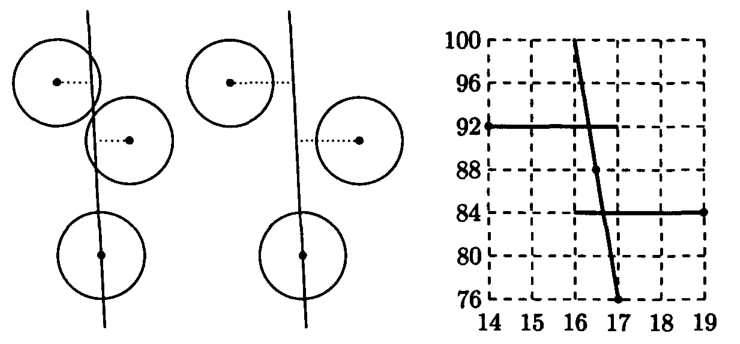
\includegraphics[scale=0.7]{hinhc6}
\end{center}
\textit{Cách làm khác.} Lưu ý rằng các đường thẳng đi qua điểm $(16,5;88)$, tâm đối xứng của hai đường tròn có tâm tại $(14;92)$ và $(19;84)$, chia diện tích của hai hình tròn này theo cách mong muốn. Do đó, đường thẳng đi qua $(16,5;88)$ và $(17;76)$ có hệ số góc là $\dfrac{88-76}{16,5-17}=-24$, chính là kết quả của bài toán. Tính duy nhất của đáp án từ việc quan sát nó cắt bán kính từ $(14;92)$ đến $(17;92)$ của một đường tròn và bán kính từ $(16;84)$ đến $(19;84)$ của đường tròn khác, được thể hiện trong hình thứ ba ở trên. (Lưu ý sự khác biệt trong quy mô.)

\textbf{Đáp án: $24$}
}%Hết câu hỏi 6

\baituluan{logic:7}{%Câu hỏi 7

Cho hàm $f$ xác định trên tập hợp các số nguyên và thỏa mãn:
\begin{center}
$
f(x)=\left\{\begin{matrix} n-3&\text{nếu } n\ge 1000.\\
f(f(n+5))&\text{nếu } n<1000.\end{matrix}\right.
$
\end{center}
Tính $f(84)$.

}{%Trả lời

Dễ dàng hơn việc tính trực tiếp $f(84)$, ta bắt đầu tính giá trị của $f(n)$ với $n=1000$ và tìm kiếm một dạng khi $n<1000$, do đó, sử dụng định nghĩa đệ quy của hàm $f$.

Thật vậy, ta có:
    \begin{align}
        \begin{split}
            f(999)=f(f(1004))=f(1001)=998,\\
            f(998)=f(f(1003))=f(1000)=997,\\
			f(997)=f(f(1002))=f(999)=998,\\
			f(996)=f(f(1001))=f(998)=997,\\
			f(995)=f(f(1000))=f(997)=998,
        \end{split}
    \end{align}
trên cơ sở đó, ta có:
    \begin{align}{f(n)=}
        \begin{cases}
            997, &\text{nếu n chẵn và } n<1000, \\
			997, &\text{nếu n lẻ và } n <1000.
        \end{cases}
    \end{align}
Để chứng minh $(4)$, rất thuận tiện khi ta sử dụng phương pháp quy nạp. Ta chứng minh $(4)$ đúng với $n$, giả sử rằng điều này đúng với mọi $m$, $n<m<1000$. Từ định nghĩa liên quan đến $f(n)$ và $f(n+5)$, ta có thể chứng minh quy nạp khi $n+5<1000$, nghĩa là, ta phải chứng minh $(4)$ đúng với $n=999;998;...;995$ riêng. Điều này đã có trong $(3)$. Bây giờ, cho $n<995$,
 \begin{align}{f(n)=f(f(n+5))=}
        \begin{cases}
            f(997)=998, &\text{nếu } n+5 \text{ chẵn}, \\
			f(997)=997, &\text{nếu } n+5 \text{ lẻ}.
        \end{cases}
    \end{align}
Lưu ý rằng $n$ chẵn khi $n+5$ lẻ và $n$ lẻ khi $n+5$ chẵn, điều phải chứng minh. Đặc biệt, từ $(4)$ ta có $f(84)=997$.

\textbf{Đáp án: $997$}
}%Hết câu hỏi 7

\baituluan{logic:8}{%Câu hỏi 8

Phương trình $z^{6}+z^{3}+1=0$ có một nghiệm phức với hệ số góc $\theta$, $90^{o}<\theta<180^{o}$ trên mặt phẳng phức. Tìm số đo của $\theta$.
}{%Trả lời

Đặt $w=z^{3}$. Khi đó, phương trình đã cho trở thành:
\begin{center}
$w^{2}+w+1=0$,
\end{center}
Phương trình trên có nghiệm là $\dfrac{-1+i\sqrt3}{2}$ và $\dfrac{-1-i\sqrt3}{2}$, với argumen lần lượt là $120^{o}$ và $240^{o}$. Từ đó, ta tìm được $6$ giá trị argumen của $z$:
    \begin{align*}
        \dfrac{120^{o}}{3}, \dfrac{120^{o}+360^{o}}{3},  \dfrac{120^{o}+720^{o}}{3},\\
		\dfrac{240^{o}}{3}, \dfrac{240^{o}+360^{o}}{3},  \dfrac{240^{o}+720^{o}}{3}.
    \end{align*}
Rõ ràng, chỉ giá trị số hai trong các giá trị trên, $160^{o}$ là nằm từ $90^{o}$ đến $180^{o}$.

\textit{Cách làm khác}. Nhân phương trình đã cho với $z^{3}-1=0$, ta được:
\begin{center}
$z^{9}-1=0$,
\end{center}
Phương trình này có $9$ nghiệm:
\begin{center}
$z_n=\cos(n.40^{o})+i\sin(n.40^{o}), n=0;1;2;...;8$.
\end{center}
Trong đó, chỉ có $z_3$ và $z_4$ là nằm trong góc phần tư thứ hai. Tuy nhiên, từ các nghiệm của phương trình $z^{9}-1=0$ phân biệt và $z_3$ là một nghiệm của phương trình $z^{3}-1=0$, ta không thể giải phương trình đã cho. Vậy nghiệm thỏa mãn là $z_4$, tức $160^{o}$.
}%Hết câu hỏi 8

\baituluan{logic:9}{%Câu hỏi 9

Cho tứ diện $ABCD$ có $AB=3cm$. Diện tích của $\triangle ABC$ và $\triangle ABD$ lần lượt là $15cm^{2}$ và $12cm^{2}$. Hai mặt phẳng $(ABC)$ và $(ABD)$ tạo với nhau một góc bằng $30^{o}$. Tính thể tích khối tứ diện $ABCD$ theo $cm^{3}$.
}{%Trả lời

Đặt $V$ là thể tích của tứ diện $ABCD$ và $h$ là chiều cao của tứ diện hạ từ $D$. Khi đó, $V=\dfrac{h.S_{ABC}}{3}$ và ta cần tìm $h$.
\begin{center}
\includegraphics[height=4cm,width=5cm]{Hinhc9}
\end{center}

Theo định nghĩa, góc $30^o$ giữa hai mặt phẳng $(ABC)$ và $ABD$ là góc giữa hai đường thẳng cắt nhau và vuông góc với giao tuyến $AB$. Chọn mặt phẳng chứa hai đường thẳng đó qua $D$ và gọi $K$, $H$ lần lượt là giao điểm của mặt phẳng này với $AB$ và mặt phẳng $(ABC)$, vì tế $DH\perp AB$. 

Từ $DK\perp AB$, ta có: 
\begin{center}
$DK=\dfrac{2.S_{ABD}}{AB}=8cm$.
\end{center}
Hơn nữa, từ $\triangle DKH$ là tam giác vuông có góc $30^o$ nên $h=DH=DK/2=4cm$. Vì vậy, thay vào công thức ở trên, ta tìm được $V=20cm^3$.

\textbf{Đáp án: $20cm^3$}

}%Hết câu hỏi 9

\baituluan{logic:10}{%Câu hỏi 10

Mary nói với John điểm của cô ấy trong kì thi American High School Math ematic Examination (AHSME) lớn hơn $80$. Theo đó, John có thể xác định được những câu Mary làm đúng. Nếu điểm của Mary thấp hơn nhưng vẫn trên $80$ thì John không thể xác định được. Hãy tìm điểm của Mary? (Lưu ý rằng AHSME gồm $30$ câu hỏi trắc nghiệm và điểm số của một người là $s$ điểm được tính bởi công thức $s=30+4c-w$, trong đó $c$ là số câu đúng và $w$ là số câu sai, học sinh không bị loại bài nếu có câu không trả lời).
}{%Trả lời

Đề bài cho $s=30+4c-w>80$ và yêu cầu tìm giá trị nhỏ nhất của $s$ tức tìm giá trị $c$ duy nhất. Trước tiên, ta thấy rằng nếu $c+w\le 25$, sau đó bằng cách tăng số câu đúng lên $1$ và số câu sai là $4$ thì số điểm nhận được như nhau. (Điều này tương đương với bất phương trình $(c+1)+(w+4)\le 30$). Vì vậy, ta phải có:
\begin{align}\label{cthuc}
c+w\ge 26.
\end{align}
và 
\begin{align}\label{cthuc}
w\le 3,
\end{align}
nếu không ta có thể giảm số câu sai bằng $4$ và số câu đúng bằng $1$, và như vậy số điểm không thay đổi. (Điều thứ hai có thể là với $s>80$ rõ ràng $c\ge 13$.) Bây giờ để tối thiểu hóa $s$, ta phải tối thiểu hóa $c$ và tối đa hóa $w$, tùy thuộc vào bất đẳng thức $(6)$ và $(7)$ ở trên. Điều này dẫn tới $w=3, c=23$ và $s=30+4.23-3=119$.

\textbf{Đáp án: 119}
}%Hết câu hỏi 10

\baituluan{logic:11}{%Câu hỏi 11

Một người làm vườn trồng ba cây táo, bốn cây sồi và năm cây bạch dương thành một hàng. Anh ấy trồng chúng một cách ngẫu nhiên và mỗi cách sắp xếp đều như nhau. Đặt $\dfrac{m}{n}$ là biến cố mà không có hai cây bạch dương liền kề với một cây bạch dương khác. Hãy tìm $m+n$. 
}{%Trả lời

$12$ cây có thể được trồng theo $12!$ cách. Đặt $k$ là biến cố sao cho không có hai cây bạch dương nào liền kề với một cây dương khác. Số cách ta có là $\dfrac{k}{12!}$. Để tìm $k$, ta phải đếm như sau:
\begin{center}
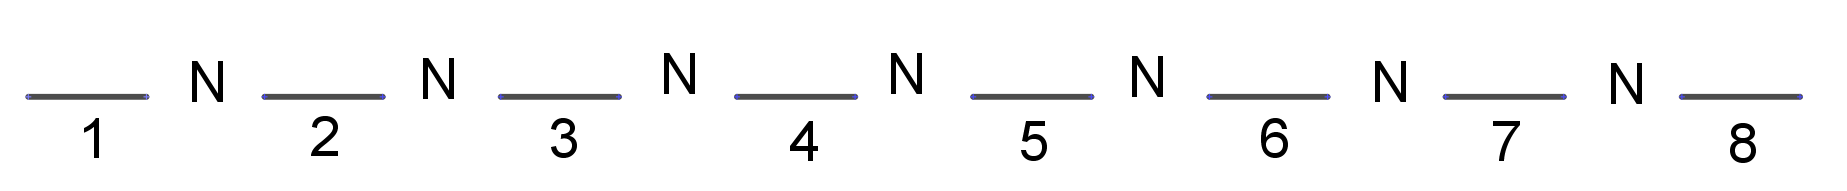
\includegraphics[scale=0.7]{hinhc11}
\end{center}
trong đó, $7$ vị trí $N$ không phải cây bạch dương và các khe từ số 1 tới số 8 được chiếm giữ bởi các cây bạch dương, mỗi cây một khe. Có $7!$ cách sắp xếp các cây không phải bạch dương và mỗi cách sắp xếp có $8.7.6.5.4$ cách sắp xếp cây bạch dương. Vì vậy, ta tìm được $k=(7!).8.7.6.5.4$, $\dfrac{m}{n}=\dfrac{(7!).8.7.6.5.4}{12!}=\dfrac{7}{99}$ và $m+n=106$.

\textit{Lưu ý.} Trong cách làm trên, ta đã giả sử mỗi cây là phân biệt. Bài toán này cũng có thể được hiểu theo nghĩa các cây phân biệt khi và chỉ khi chúng khác loài. Trong trường hợp này, các phép t (nghĩa là tử số và mẫu số) là khác nhau nhưng xác suất hóa ra lại như nhau.

\textbf{Đáp án: 106}
}%Hết câu hỏi 11

\baituluan{logic:12}{%Câu hỏi 12

Cho hàm $f$ xác định trên tập số thực và thỏa mãn:
\begin{center}
$f(2+x)=f(2-x)$ và $f(7+x)=f(7-x)$
\end{center}
với mọi số thực $x$. Nếu $x=0$ là một nghiệm của $f(x)=0$ thì có ít nhất bao nhiêu nghiệm của $f(x)=0$ thỏa mãn $-1000\le x\le 1000$?
}{%Trả lời

Đầu tiên, ta sử dụng các phương trình đã cho để tìm các biến số trên tập xác định mà $f$ gán giá trị giống nhau. Ta có:
\begin{align}\label{cthuc}
f(x)=f(2+(x-2))=f(2-(x-2))=f(4-x)
\end{align}
và 
\begin{align}\label{cthuc}
f(4-x)=f(7-(x+3))=f(7+(x+3))=f(x+10).
\end{align}
Từ phương trình $(8)$ và $(9)$ ta có:
\begin{align}\label{cthuc}
f(x+10)=f(x)
\end{align}
Thay $x$ bằng $x+10$ và sau đó là $x-10$ trong phương trình $(10)$, ta nhận được $f(x+10)=f(x+20)$ và $f(x-10)=f(x)$. Tiếp tục cách này, ta có:
\begin{align}\label{cthuc}
f(x+10n)=f(x), với n=\pm 1, \pm 2, \pm 3, ...
\end{align}
Vì $f(0)=0$, phương trình $(11)$ có nghĩa là:
\begin{center}
$f(\pm 10)=f(\pm 20)=...=f(\pm 1000)=0$,
\end{center}
cần tổng $201$ nghiệm của phương trình $f(x)=0$ trong khg $[-1000;1000]$.

Tiếp theo ta đặt $x=0$ trong phương trình $(8)$, theo đó$f(4)=f(0)=0$. Đặt $x=4$ trong phương trình $(11)$, ta được nhiều hơn $200$ nghiệm của $f(x)=0$ với $x=-996; -986;...;-6;4;14;...;994$. Vì hàm zig-zag trong hình phía dưới thỏa mãn điều kiện và có chính xác những nghiệm đó, do vậy đáp án của bài toán là $401$.
\begin{center}
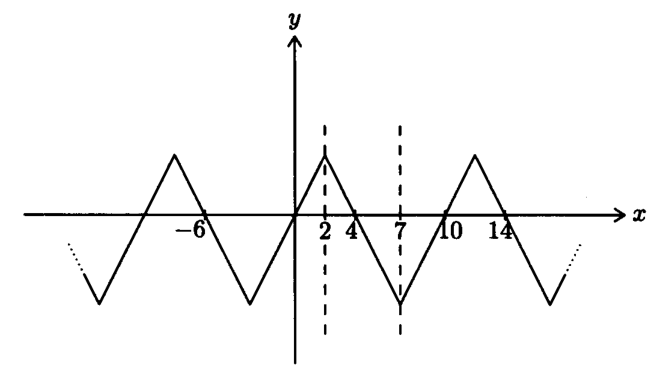
\includegraphics[scale=0.7]{hinhc12}
\end{center}

\textbf{Đáp án: 401}
}%Hết câu hỏi 12

\baituluan{logic:13}{%Câu hỏi 13

Tính giá trị của biểu thức: 
\begin{center}
$10\cot(\cot^{-1}3+\cot^{-1}7+\cot^{-1}13+\cot^{-1}21)$.
\end{center}
}{%Trả lời

Để đơn giản biểu thức đã cho, ta đặt
\begin{align}\label{cthuc}
a=\cot^{-1}3, \hspace{0.1cm} b=\cot^{-1}7, & \hspace{0.1cm} c=\cot^{-1}13, \hspace{0.1cm} d=\cot^{-1}21,\\
e=a+b \hspace{0.1cm}& \text{và } f=c+d
\end{align}
Từ $(12)$ và $(13)$, bài toán tương đương với tìm giá trị của $10\cot(e+f)$.
Dễ dàng chứng minh được:
\begin{align}\label{cthuc}
\cot(x+y)=\dfrac{\cot x.\cot y - 1}{\cot x+\cot y}.
\end{align}
Hơn nữa, ngay cả khi $\cot^{-1}$ được xem là một hàm nhiều giá trị,
\begin{align}\label{cthuc}
\cot(\cot^{-1}x)=x, \text{với mọi số thực x}.
\end{align}
Ta giải các phương trình từ $(12)$ đến $(15)$ ở trên, ta được:
    \begin{align*}
        \cot e=\cot (a+b)&=\dfrac{3\cdot7 - 1}{3+7}=2,\\
        \cot f = \cot (c+d)&=\dfrac{13\cdot21- 1}{3+21}=8,\\
        \cot (e+f)&=\dfrac{2\cdot8- 1}{2+8}=\dfrac{3}{2},
    \end{align*}
và từ đó, $10\cot (e+f)=15$ là đáp án của bài toán.

\textbf{Đáp án: 15}
}%Hết câu hỏi 13

\baituluan{logic:14}{%Câu hỏi 14

Tìm số nguyên chẵn lớn nhất không thể viết thành tổng của hai hợp số lẻ? (Lưu ý rằng một số nguyên dương được gọi là hợp số nếu nó chia hết cho một số nguyên dương khác $1$ và chính nó.)
}{%Trả lời

Ta sẽ chứng minh rằng nếu $k$ là số nguyên chẵn và $k\ge 40$ thì $k$ được biểu diễn thành tổng của hai hợp số. Theo đó, $38$ là một số nguyên chẵn lớn nhất không thể biểu thị theo cách đó; thật dễ dàng để kiểm tra điều này. Mục tiêu chứng minh của ta với $k\ge 40$ thực tế là nếu $n$ lẻ và lớn hơn $1$ thì $5n$ là hợp số lẻ kết thúc bằng chữ số $5$. Vì vậy, để biểu diễn $k$ như mong muốn, ta cần tìm hợp số lẻ nhỏ kết thúc bằng chữ số $5, 7, 9, 1$ và $3$ và thêm chúng vào số có dạng $5n$. Thật vậy, $15, 27, 9, 21$ và $33$ thỏa mãn những điều kiện trên và trong mỗi trường hợp sau đây, người ta có thể tìm số nguyên lẻ $n$, $n>1$ sao cho:
  \begin{align*}
       \text{Nếu} \hspace{0.1cm} k \hspace{0.1cm} \text{kết thúc bằng} &\hspace{0.1cm} 0 \hspace{0.1cm} (\text{tức là}\hspace{0.1cm} 40, 50, ...)\text{thì} \hspace{0.1cm} k=15+5n,\\
        \text{Nếu} \hspace{0.1cm} k \hspace{0.1cm} \text{kết thúc bằng} &\hspace{0.1cm} 2 \hspace{0.1cm} (\text{tức là} \hspace{0.1cm}42, 52, ...)\text{thì} \hspace{0.1cm} k=27+5n,\\
        \text{Nếu} \hspace{0.1cm} k \hspace{0.1cm} \text{kết thúc bằng} &\hspace{0.1cm} 4 \hspace{0.1cm} (\text{tức là} \hspace{0.1cm}44, 54, ...)\text{thì} \hspace{0.1cm} k=9+5n,\\
       \text{Nếu} \hspace{0.1cm} k \hspace{0.1cm} \text{kết thúc bằng} &\hspace{0.1cm} 6 \hspace{0.1cm} (\text{tức là} \hspace{0.1cm}46, 56, ...)\text{thì} \hspace{0.1cm} k=21+5n,\\
       \text{Nếu} \hspace{0.1cm} k \hspace{0.1cm} \text{kết thúc bằng} &\hspace{0.1cm} 8 \hspace{0.1cm} (\text{tức là}\hspace{0.1cm} 48, 58, ...)\text{thì} \hspace{0.1cm} k=33+5n.\\
    \end{align*}

\textbf{Đáp án: 38}
}%Hết câu hỏi 14

\baituluan{logic:15}{%Câu hỏi 15

Tính $x^{2}+y^{2}+z^{2}+w^{2}$ nếu:
    \begin{align*}
        \dfrac{x^{2}}{2^{2}-1^{2}} +\dfrac{y^{2}}{2^{2}-3^{2}}+\dfrac{z^{2}}{2^{2}-5^{2}}+\dfrac{w^{2}}{2^{2}-7^{2}}&=1,\\
         \dfrac{x^{2}}{4^{2}-1^{2}} +\dfrac{y^{2}}{4^{2}-3^{2}}+\dfrac{z^{2}}{4^{2}-5^{2}}+\dfrac{w^{2}}{4^{2}-7^{2}}&=1,\\
       \dfrac{x^{2}}{6^{2}-1^{2}} +\dfrac{y^{2}}{6^{2}-3^{2}}+\dfrac{z^{2}}{6^{2}-5^{2}}+\dfrac{w^{2}}{6^{2}-7^{2}}&=1,\\
  \dfrac{x^{2}}{8^{2}-1^{2}} +\dfrac{y^{2}}{8^{2}-3^{2}}+\dfrac{z^{2}}{8^{2}-5^{2}}+\dfrac{w^{2}}{8^{2}-7^{2}}&=1.   
\end{align*}
}{%Trả lời

Khẳng định rằng hệ phương trình đã cho thỏa mãn với $x^{2}, y^{2}, z^{2}$ và $w^{2}$ tương đương với phương trình:
\begin{align}\label{cthuc}
\dfrac{x^{2}}{t-1}+\dfrac{y^{2}}{t-9}+\dfrac{z^{2}}{t-25}+\dfrac{w^{2}}{t-49}=1
\end{align}
thỏa mãn với $t=4, 16, 36$ và $64$. Quy đồng mẫu số phương trình $(16)$ với mọi $t\ne 1, 9, 25, 49$, ta được phương trình tương đương:
\begin{multline}\label{cthuc}
(t-1)(t-9)(t-25)(t-49)-x^{2}(t-9)(t-25)(t-49)\\
-y^{2}(t-1)(t-25)(t-49)-z^{2}(t-1)(t-9)(t-49)-w^{2}(t-1)(t-9)(t-25)=0,
\end{multline}
trong đó, vế trái là đa thức bậc bốn ẩn $t$. Vì $t=4, 16, 36$ và $64$ được coi là nghiệm và đa thức bậc bốn có tối đa bốn nghiệm nên tất cả những giá trị đó của $t$ là nghiệm. Theo đó, $(17)$ tương đương với phương trình:
\begin{align}\label{cthuc}
(t-4)(t-16)(t-36)(t-64)=0.
\end{align}
Vì hệ số của $t^{4}$ là $1$ trong cả phương trình $(17)$và $(18)$ nên người ta có thể kết luận rằng hệ số của các lũy thừa của $t$ cũng phải giống nhau. Cụ thể, cân bằng hệ số của $t^{3}$, ta có:
\begin{center}
$1+9+25+49+x^{2}+y^{2}+z^{2}+w^{2}=4+16+36+64$,
\end{center}
Từ đó, $x^{2}+y^{2}+z^{2}+w^{2}=36$.

\textbf{Đáp án: 36}
}%Hết câu hỏi 15


%%16:11:43 26/6/2019Last Modification of contents
%%17:29:58 27/6/2019Last Modification of contents